\documentclass{article}\usepackage[]{graphicx}\usepackage[]{color}
%% maxwidth is the original width if it is less than linewidth
%% otherwise use linewidth (to make sure the graphics do not exceed the margin)
\makeatletter
\def\maxwidth{ %
  \ifdim\Gin@nat@width>\linewidth
    \linewidth
  \else
    \Gin@nat@width
  \fi
}
\makeatother

\definecolor{fgcolor}{rgb}{0.345, 0.345, 0.345}
\newcommand{\hlnum}[1]{\textcolor[rgb]{0.686,0.059,0.569}{#1}}%
\newcommand{\hlstr}[1]{\textcolor[rgb]{0.192,0.494,0.8}{#1}}%
\newcommand{\hlcom}[1]{\textcolor[rgb]{0.678,0.584,0.686}{\textit{#1}}}%
\newcommand{\hlopt}[1]{\textcolor[rgb]{0,0,0}{#1}}%
\newcommand{\hlstd}[1]{\textcolor[rgb]{0.345,0.345,0.345}{#1}}%
\newcommand{\hlkwa}[1]{\textcolor[rgb]{0.161,0.373,0.58}{\textbf{#1}}}%
\newcommand{\hlkwb}[1]{\textcolor[rgb]{0.69,0.353,0.396}{#1}}%
\newcommand{\hlkwc}[1]{\textcolor[rgb]{0.333,0.667,0.333}{#1}}%
\newcommand{\hlkwd}[1]{\textcolor[rgb]{0.737,0.353,0.396}{\textbf{#1}}}%
\let\hlipl\hlkwb

\usepackage{framed}
\makeatletter
\newenvironment{kframe}{%
 \def\at@end@of@kframe{}%
 \ifinner\ifhmode%
  \def\at@end@of@kframe{\end{minipage}}%
  \begin{minipage}{\columnwidth}%
 \fi\fi%
 \def\FrameCommand##1{\hskip\@totalleftmargin \hskip-\fboxsep
 \colorbox{shadecolor}{##1}\hskip-\fboxsep
     % There is no \\@totalrightmargin, so:
     \hskip-\linewidth \hskip-\@totalleftmargin \hskip\columnwidth}%
 \MakeFramed {\advance\hsize-\width
   \@totalleftmargin\z@ \linewidth\hsize
   \@setminipage}}%
 {\par\unskip\endMakeFramed%
 \at@end@of@kframe}
\makeatother

\definecolor{shadecolor}{rgb}{.97, .97, .97}
\definecolor{messagecolor}{rgb}{0, 0, 0}
\definecolor{warningcolor}{rgb}{1, 0, 1}
\definecolor{errorcolor}{rgb}{1, 0, 0}
\newenvironment{knitrout}{}{} % an empty environment to be redefined in TeX

\usepackage{alltt}
\usepackage{geometry}
\usepackage[round]{natbib}
\bibliographystyle{abbrvnat}
\usepackage{graphicx}
\geometry{a4paper}
\usepackage[T1]{fontenc}
\usepackage[utf8]{inputenc}
\usepackage{authblk}
\usepackage[running]{lineno}
\usepackage{setspace}
\usepackage{courier}
\usepackage{tabulary}
\usepackage{hyperref}
\doublespacing

\newcommand{\tom}[1]{{\textit{\color{red}{[#1]}}}}
\newcommand{\aldo}[1]{{\textit{\color{blue}{[#1]}}}}

\title{\texttt{popler}: An R package for synthesis of population time series from long-term ecological research}
\author[a,b,c]{Aldo Compagnoni\thanks{aldo.compagnoni@gmail.com}}
\author[a]{Andrew J. Bibian}
\author[a]{Brad M. Ochocki}
\author[b,c]{Sam Levin}
\author[d]{Margaret O'Brien}
\author[e]{Kai Zhu}
\author[a]{Tom E.X. Miller}

\affil[a]{Department of BioSciences, Program in Ecology and Evolutionary Biology, Rice University, 6100 Main St, MS-170, Houston, TX 77005}
\affil[b]{Institute of Biology, Martin Luther University Halle-Wittenberg, Am Kirchtor 1, 06108 Halle (Saale), Germany}
\affil[c]{German Centre for Integrative Biodiversity Research (iDiv) Halle-Jena-Leipzig, Deutscher Platz 5e, 04103 Leipzig, Germany}
\affil[d]{Marine Science Institute, University of California, Santa Barbara, CA 93016, United States}
\affil[e]{Department of Environmental Studies, University of California, Santa Cruz, CA 95064, USA}

\renewcommand\Authands{ and }
\date{Running headline: The \texttt{popler} database and R package}
\IfFileExists{upquote.sty}{\usepackage{upquote}}{}
\begin{document}



\maketitle
\tom{Tom's comments appear in red italics.}
\aldo{Aldo's comments appear in blue italics.}

\newpage

\section*{Abstract}
%The Abstract must not exceed 350 words and should list the main results and conclusions, using simple, factual, numbered statements: Point 1: set the context for and purpose of the work; Point 2: indicate the approach and methods; Point 3: outline the main results; Point 4: identify the conclusions and the wider implications.

\begin{enumerate}

  \item Population dynamics has a central role in the historical and current development of both fundamental and applied ecological science. The nascent culture of open data promises to increase the value of population dynamics studies to the field of ecology. However, users interested in data synthesis using population data are stymied by the difficulty in identifying relevant datasets, and by the heterogeneity of the available data.
  
  \item To obviate these issues, we built a relational database, popler, and an \texttt{R} package, library("popler"), designed to interact with it. popler accommodates the vast majority of population data under a common structure, and without the need for aggregating raw observations. library("popler") is  designed for users unfamiliar with the SQL language and with the structure of the database. This \texttt{R} library allows users to identify, download, explore, and cite datasets salient to their needs.

  \item We implemented popler as a PostgreSQL instance, where we stored population data originated by the United Stated Long Term Ecological Research (LTER) Network. Our focus on the US LTER data aims to leverage the untapped potential of this vast open data resource. The database currently contains 275 datasets from 25 LTER sites. \aldo{report number of datasets, taxa, number of observations}
  
  \item The combination of the online database and the \texttt{R} library("popler") is a resource to data synthesis efforts in population ecology. The common structure of popler simplifies comparative analyses, and the availability of raw data confers the largest freedom when exploiting datasets. library("popler") maximizes these opportunities by providing a user-friendly interface to the online database.

   \end{enumerate}
\section*{Keywords}
\linenumbers
open long-term population data, US Long Term Ecological Research Network data, online database, database structure, PostgreSQL, R package, data synthesis, comparative analysis

\newpage
\section*{Introduction}
\linenumbers

Population dynamics – changes in species’ abundance and composition through time and space – are central to ecology for both applied and fundamental reasons. Population studies are a standard tool in conservation, particularly to perform risk assessment and viability analysis \citep{Morris2002b,Beissinger2002}. Population studies are also an integral part of fundamental ecological research. Populations are the building blocks of ecological dynamics at higher scales of organization, and examples abound showing how the study of population ecology improves understanding in evolution \citep{Metcalf2007}, community ecology \citep{Levine2009}, and ecosystem ecology \citep{Medvigy2009,Fisher2018}.

Given their central role in ecology, studies of population dynamics will be an essential component in the advances allowed by the flourishing culture of open access and data synthesis. The increase in freely available ecological data sets is poised to change ecological science \citep{Laurance2016}. The rising focus on open data is clear in changing publishing standards, in the design of observational networks like the National Ecological Observatory Network \citep{schimel2007neon}, and in the online availability of previously proprietary data \citep{Kratz2003,Bechtold2005}. This deluge of open data holds tremendous promise to facilitate comparative analyses and to test the generality of ecological hypotheses. For population dynamics in particular, it is the increasing availability of long-term data that will likely yield the most substantial scientific advances, as long time series are required to detect trends in abundance \citep{Lindenmayer2012}, quantify temporal variance \citep{Compagnoni2016}, and identify endogenous \citep{Knape2012} or exogenous \citep{Knape2011,Hampton2013} drivers of population fluctuations.

There is ample evidence demonstrating the importance of long-term data for population ecology to facilitate comparative and synthetic studies \citep{Lindenmayer2012,Giron-Nava2017}. To our knowledge, there is currently just one publicly accessible database focused on long-term population dynamics: the Global Population Dynamics Database \citep[GPDD,][]{Inchausti2001}. The GPDD provides over 5000 time series of population size longer than 10 years for over 1800 animal species. This database has been powerfully leveraged for comparative analyses and syntheses \citep[e.g.,][]{Knape2012} but it has some important limitations. GPDD time series are not spatially replicated – there is one observation of population size or density temporal replicate, with no estimate of uncertainty – making it difficult or impossible to isolate different sources of variability and requiring the assumption that population size is known without error. Retaining information on spatial replication would expand the variety of research questions that can be asked and improve estimation of uncertainty in the answers. Additionally, the GPDD focuses exclusively on single species dynamics, making it difficult or impossible to link the dynamics of multiple fluctuating populations within ecological communities \citep[e.g.,][]{Ushio2018}.  

One of the best sources of publicly available long-term observations of population abundance of diverse plants and animals is the Long-Term Ecological Research (LTER) network supported by the U.S. National Science Foundation. The LTER was founded in 1980 and grew from the original six sites to the current 28 sites throughout North America plus one each in Puerto Rico and Antarctica. Synthetic and comparative studies from the LTER network have made valuable contributions to ecological understanding \citep{Knapp2012}. However, the majority of LTER synthesis research has focused on ecological dynamics at the community (e.g. \cite{Wilcox2017}) and ecosystem (e.g. \cite{Knapp2001}) scales. Nevertheless, every LTER site collects population abundance data as one of its five core areas of continuous observations \citep{Callahan1984}. These population time series include both single- and multi-species studies. In our opinion, these data, which have been accumulating since 1980, are under-used. One issue that may limit the use of LTER population data in synthetic, comparative studies is their heterogeneity. Indeed, several authors have noticed that progress in ecology is hindered by difficulties in the way data is accessed, by heterogeneities in the way data is structured, and by failure to cite data originators \tom{Jones et al. 2004, Reichman et al. 2011}. The structure of LTER data sets may be widely different, employing a variety of data types (counts of individuals, biomass estimates, percent cover, etc.), experimental designs driven by the priorities of particular PIs, and diverse replication schemes – idiosyncrasies that may be difficult to accommodate in a one-size-fits-all database. However, these challenges also present valuable opportunities. For example, the hierarchical replication structure of many LTER studies (e.g., subplots within plots within transects) can facilitate more sophisticated statistical investigation than would be possible with simpler, aggregated, or unreplicated data. %Ad-hoc software can greatly aid the discovery, querying, and comparison of datasets (e.g. \cite{Morris2013}). Dedicated software is therefore important to maximize the fruition, and the ultimate impact of publicly available datasets.

To overcome the issues posed by heterogeneous data structures, we developed \texttt{popler} (POPulation dynamics in Long-term Ecological Research), an online database of LTER population studies. We also developed a companion R package to aid in discovery, querying, and synthesis. The \texttt{popler} database defines a common data structure to accommodate nearly every long-term population data set provided by the LTER network as of this writing. The common data structure facilitates the identification, access, and manipulation of raw population data through a user-friendly R package. Our goals here are to provide introductions to the \texttt{popler} database and R package, which we believe will be useful resources in population, community, and macro ecology. Our focus here is on LTER time series but our database schema can in principle, accommodate any population level dataset and expanding popler beyond the LTER network is a priority for future development.

\section*{The \texttt{popler} database}
\texttt{popler} aims to organize population data from the LTER network using a common structure. To achieve this, we identified a set of variables relevant to population studies (Table \ref{Tab:vars}) and organized them into a relational database (Fig. \ref{Fig:schema}). In \texttt{popler}, we store ``raw'' data, meaning that we have not modified or aggregated the original observations. Our goal was to organize data under a common structure. If needed, this structure facilitates downstream aggregation and subsetting of the original data.

\subsection*{Population data}
Time series of population size are the heart of the \texttt{popler} database. We defined `population data' as time-series of observations on the size or density of a population of a species or other taxonomic unit. Observations of population size are stored in a variable called \texttt{abundance\textunderscore observation} and can be measured as a count, biomass, density, or cover. Counts and biomass are absolute measures, density is a measure of population size taken with respect to a one-, two-, or three-dimensional unit of observation, and cover is a relative (e.g., percentage) or absolute (e.g., area) measure. These four types of population data are stored in the homonymous tables of the database (Fig. \ref{Fig:schema}A).

The population datasets contained in popler are always replicated temporally. Temporal replicates are identified with up to three variables: \texttt{year}, \texttt{month}, and \texttt{day}. In theory, population data can be collected at a smaller temporal resolution (e.g. hourly). However, we did not encounter LTER datasets whose sampling was more frequent than daily. 

Population data are also almost always spatially replicated. Hence, they provide measures of population abundance at multiple locations. Furthermore, spatial replicates are often nested, where for example a study might be replicated at separate sites (e.g. a watershed, a lake, an island, etc.), each of which contains intermediate spatial replicates (e.g. a transect, a block), which in turn contain the smallest spatial replicate at which observations are made (e.g. a plot, a quadrat). The hypothetical study described above would have three nested levels of spatial replication, identified by three numbered \texttt{spatial replication} variables. In \texttt{popler}, we accommodate data sets with up to five spatial replication levels (Table \ref{Tab:vars}). For simplicity, we call the first, and therefore largest spatial replicate ``study site'' (Fig. \ref{Fig:schema}C). This is not the LTER site, one of the 28 NSF-supported locations (Table \ref{Tab:S3}).

\texttt{popler} contains both observational and experimental studies. Experimental datasets contained information on one or more experimental treatments. Popler accommodates information on up to three experimental treatments, identified by three numbered \texttt{treatment type} variables (Table \ref{Tab:vars}). 

Most datasets contain one or more variables in addition to the ones described above which we store in a list of variable called \texttt{covariates}. Covariates might report, for example, the hour of day or the temperature when population data was collected, the Cartesian coordinates of spatial replicates, and so on. Covariates can be useful for time series that contain information on population structure \tom{Would this be indicated in the metadata? How would someone search for such studies or know if they are working with one?}. In these datasets, population size refers to subdivisions of the entire population, such as males and females, large and small individuals, developmental different stages, and so forth.

Finally, in addition to time series of abundance, \texttt{popler} contains individual-level data. This data provide information on the attributes of the individuals, or a subset thereof, that make up a population. We store this information in a dedicated table ("Individual", Fig. \ref{Fig:schema}A). As individual attributes we consider variables that describe identity, size, sex, life stage (e.g. instar versus adult in insects) or status (e.g. reproductive or non-reproductive, live or dead). We refer to these individual attributes with the term ``structure'': \texttt{popler} accommodates data sets that measure up to four types of structure simultaneously. We store these data in up to four numbered \texttt{structure\textunderscore type} variables. While these data are not population time series, we chose to include them in \texttt{popler} because they provide information on demographic transitions that can be used to derive estimates of population growth. Moreover, in the cases of datasets that sample all of the individuals in a population, individuals can be aggregated (i.e. summed) as a measure of population size.

\subsection*{Taxonomic information}
Each observation of abundance or individual state corresponds to a taxonomic unit (Fig. \ref{Fig:schema}B). Population data typically refer to a species or a genus, but we also include data that refer to a higher taxonomic rank, such as family, or order. %The majority of data sets provided by the LTER include multiple taxa, so each observation regarding population size or individual attribute is associated with a unique taxonomic unit.--seems redundant
Popler provides 15 taxonomic ranks, and two additional variables that refer to how taxonomic information is recorded in the original datasets. The additional variables are \texttt{sppcode}, which are taxon-specific alphanumeric codes, and \texttt{common\textunderscore name}, the common name of each taxonomic unit (Table S1).

Popler stores the taxonomic information linked to each study in two tables: one containing the original taxonomic information reported by the PI, the other containing the accepted taxonomic information derived from the former (Fig. \ref{Fig:schema}B). Raw taxonomic data typically contains ambiguities derived by the dynamic changes in species classifications \citep{Chamberlain2013}. The raw data also typically fail to include higher-level taxonomic information above the genus level. To provide as much taxonomic information as possible, \texttt{popler} provides a second table linking taxonomic units provided by the authors to accepted taxonomic units according to the algorithms provided by the R package \texttt{taxize} \citep{Chamberlain2013}. This package links taxon names to the unambiguous entry of an online taxonomic database.

\subsection*{Study site}
We stored the locations of datasets by recording the latitude (\texttt{lat\textunderscore study\textunderscore site}) and longitude (\texttt{lng\textunderscore study\textunderscore site}) of study sites (Fig. \ref{Fig:schema}C). Storing this information in a separate table allows for explicit connections between independent data sets collected at the same locations within LTER sites. We emphasize that ``study sites'' refer to the first and therefore largest level of nested spatial replication. These study sites are at a smaller scale than ``LTER sites'' (the 28 NSF-supported locations; Table A1).

\subsection*{Metadata}
The metadata table describes 48 variables (Table S2) with general information about the dataset, its temporal and spatial replication, and its study design (Fig. \ref{Fig:schema}D). The general information includes a title designated by the original authors, link to online metadata, contact information for data originators, and the type of data provided by the dataset (i.e., which of the five tables in Fig. \ref{Fig:schema}A the data is stored in).

All remaining metadata is related to the variables stored in the tables of \ref{Fig:schema}A and \ref{Fig:schema}B. These metadata provide information on temporal replication, spatial replication, and study design. First, we providethe years elapsed between the first and last observation (\texttt{duration\textunderscore years}), and the sampling frequency (\texttt{samplefreq}). We report the prevalent sampling frequency, because in most datasets sampling changes during the length of the study. These metadata relate to the variables \texttt{day}, \texttt{month}, \texttt{year} of the original datasets (Table \ref{Tab:vars}). Second, we quantify spatial replication providing the number of levels of nested spatial replicates, and with the number of replicates for each spatially nested level. These metadata relate to \texttt{spatial\textunderscore replicate\textunderscore n} of the original datasets. Third, we provide basic information on the design of the study that originated each dataset. We show whether studies focus on a single species or on multiple species through \texttt{community}. This variable indicates whether the taxonomic tables (\ref{Fig:schema}B) contain more than one taxa. Studies can also be observational or experimental (\texttt{studytype}). If a study is experimental, we provide information on the type of treatments imposed by the study (\texttt{treatment\textunderscore type\textunderscore n}) and, when available, which is the control treatment (\texttt{control\textunderscore group}). The (\texttt{studytype}) variable refers to variables \texttt{treatment\textunderscore type\textunderscore n} in the original datasets. Finally, when abundance data stored in the \texttt{abundance\textunderscore observation} variable is aggregated across space or time, rather than raw, we consider these data as derived (\texttt{derived}).

\subsection*{Creation and contents of the \texttt{popler} database}
We implemented \texttt{popler} as an instance of PostgreSQL 9.2.18. We selected the candidate datasets online, pre-processed the associated files, and uploaded them in the database through a graphic user interface we developed in Python. We selected the candidate datasets by scraping information from the internet sites associated with each one of the 28 LTER sites (Table A1). We scraped this data using libraries scrapy in Python, and rvest and RSelenium in R.

We included or excluded studies based on several criteria. First, we only included studies that reported repeated observations of populations or individuals through time. Second, we included studies with at least five years of data. We performed this selection in early 2017, so datasets that are not currently stored in \texttt{popler} might now meet this criterion. We did not require population censuses to be consecutive (some studies have an irregular sampling frequency). Third, we selected only datasets for which the observations had corresponding taxonomic information, which implies that we ignored time series data on species richness or on the abundance of functional types.

%In several cases, we integrated the taxonomic information provided in the original datasets, which only reported alphanumeric species codes. We obtained taxonomic information from a separate file, from the online dataset documentation or, more rarely, from emailing the dataset originator. 
Before uploading to the online database, we preprocessed datasets in python and R. We often had to combine the separate files associated with the same dataset, transform datasets from ``wide'' to ``long'' form, convert non-ASCII characters, and handling ambiguous study sites. We provide the details of this pre-processing in Appendix S1.


The \texttt{popler} database resulting from this process contains data from 274 studies (118 of which are experimental) representing 3613 cumulative years of observations with a mean study duration of 13.19 years. \texttt{popler} contains data from 691 plant species, 349 animal species, and 1 fungal species.

\section*{The \texttt{popler} package}
The \texttt{popler} R package consists of three core functions that allow users to browse and retrieve data from the database (Fig. \ref{Fig:pack_funs}). In order of intended use, these functions are: \texttt{dictionary()}, \texttt{browse()}, and \texttt{get\textunderscore data()}. This order of use revolves around a summary table made up of the variables contained in the metadata (Fig. Fig. \ref{Fig:schema}D) and taxonomic (Fig. Fig. \ref{Fig:schema}B) tables of the online database. Each row of the summary table corresponds to a dataset and each column corresponds to one of the metadata variables that describe it. The \texttt{dictionary()} function explains what these variables (or columns) are, and it shows their content. This content provides the information needed to subset and visualize metadata through the \texttt{browse()} function, which returns studies (or rows) that satify the subset criteria. Finally, following exploration of the metadata, raw data can be downloaded with the \texttt{get\textunderscore data()} function. Below we describe these functions and illustrate their use in greater detail.

\subsection*{The \texttt{dictionary()} function}
The dictionary function is a good place for new users to begin working with \texttt{popler} (Fig. \ref{Fig:pack_funs}). With no arguments provided, this function returns a subset of the most useful metadata variables associated with each  dataset (Fig. \ref{Fig:schema}):
\begin{knitrout}
\definecolor{shadecolor}{rgb}{0.969, 0.969, 0.969}\color{fgcolor}\begin{kframe}
\begin{verbatim}
##             variable                                 description
## 1              title                            title of project
## 2  proj_metadata_key                           unique project id
## 3             lterid                                   lter name
## 4           datatype type of abundance data (e.g. count,biomass)
## 5          studytype        experimental or observational study?
## 6     duration_years                duration of project in years
## 7          community        does data set contain multiple taxa?
## 8          structure               types of indidivual structure
## 9          treatment                          types of treatment
## 10          lat_lter                          lter site latitude
## 11          lng_lter                         lter site longitude
## 12           species        specific epithet of a taxonomic unit
## 13           kingdom                                     kingdom
## 14            phylum                                      phylum
## 15             class                                       class
## 16             order                                       order
## 17            family                                      family
## 18             genus                                       genus
\end{verbatim}
\end{kframe}
\end{knitrout}
Setting argument \texttt{full\textunderscore tbl} to \texttt{TRUE} returns all 76 metadata variables. Each one of these variables name can be provided as an argument to \texttt{dictionary()}, which will then return the possible unique values of the variable. For example, \texttt{dictionary(lterid)} returns the three letter codes for all sites in the LTER network, \texttt{dictionary(genus)} returns all the genera represented in the database, etc. This output provides the starting point for developing criteria with which to identify relevant datasets.

\subsection*{The \texttt{browse()} function}
Once the user is familiar with the meaning and content of the variables that define \texttt{popler} datasets, they are ready to dig deeper using \texttt{browse()} (Fig. \ref{Fig:pack_funs}). Running \texttt{browse()} without arguments provides the metadata from all of the datasets currently stored in popler. This will be a $274 * 19$ data frame, with each row corresponding to a study and each column corresponding to a variable defined by \texttt{dictionary()}.

The full strength of \texttt{browse()} is achieved by subsetting studies according to desired criteria using standard logical expressions. For example, the user might want to consider only studies whose duration is 30 years or greater, which can be subsetted with:
\begin{knitrout}
\definecolor{shadecolor}{rgb}{0.969, 0.969, 0.969}\color{fgcolor}\begin{kframe}
\begin{alltt}
\hlstd{LTER_30} \hlkwb{<-} \hlkwd{browse}\hlstd{( duration_years} \hlopt{>} \hlnum{29}\hlstd{)}
\end{alltt}
\end{kframe}
\end{knitrout}
This operation will create the object \texttt{LTER\textunderscore 30}, which provides metadata for the data sets that satisfy the specified criterion. Multiple criteria may be combined. For example, 30+ year studies of plants can be browsed with
\begin{knitrout}
\definecolor{shadecolor}{rgb}{0.969, 0.969, 0.969}\color{fgcolor}\begin{kframe}
\begin{alltt}
\hlstd{LTER_30_plants} \hlkwb{<-} \hlkwd{browse}\hlstd{( duration_years} \hlopt{>} \hlnum{29} \hlopt{&} \hlstd{kingdom} \hlopt{==} \hlstr{"Plantae"}\hlstd{)}
\end{alltt}
\end{kframe}
\end{knitrout}
It is at the \texttt{browse()} stage that users should  vet the data sets that meet their criteria. To facilitate data exploration, \texttt{browse()} output can be printed in a more readable settings by providing \texttt{report = TRUE} as an argument, which opens up a formatted html document (Fig. \ref{Fig:reportT}). The metadata provided by \texttt{browse()} not only contains information on the characteristics of a study but also information on how to cite the study, its unique identifiers, including doi, Knowledge Network for Biocomplexity (\url{http://knb.ecoinformatics.org}) catalog system identifier, the contact information of study PIs, and a hyperlink to the url providing the original data.


\subsection*{The \texttt{get\textunderscore data()} function}

Once data sets of interest have been identified, \texttt{get\textunderscore data()} downloads the data from a server that hosts the database. This function can take as its first argument a \texttt{browse} object, a logical expression, either, or both. For example, %I set eval to false in these chunks because they each take a long time to run. I ran them once in R.
\begin{knitrout}
\definecolor{shadecolor}{rgb}{0.969, 0.969, 0.969}\color{fgcolor}\begin{kframe}
\begin{alltt}
\hlstd{LTER_30_dat} \hlkwb{<-} \hlkwd{get_data}\hlstd{(LTER_30)}
\end{alltt}
\end{kframe}
\end{knitrout}
downloads the raw data from the studies described in the browse object \texttt{LTER\textunderscore 30} and 
\begin{knitrout}
\definecolor{shadecolor}{rgb}{0.969, 0.969, 0.969}\color{fgcolor}\begin{kframe}
\begin{alltt}
\hlstd{BNZ_30_dat} \hlkwb{<-} \hlkwd{get_data}\hlstd{(LTER_30,lterid} \hlopt{==} \hlstr{"BNZ"}\hlstd{)}
\end{alltt}
\end{kframe}
\end{knitrout}
downloads the subset of data sets in \texttt{LTER\textunderscore 30} from the Bonanza Creek LTER site. The three letter code ``BNZ'' could have been located running \texttt{dictionary(lterid)} (we show the meaning of three letters codes in Table S3). The data downloaded from \texttt{popler} are in ``long'' form, meaning that each row of data reports a single measure of population size, and separate variables indicate the temporal and spatial replicate, taxonomic information, etc. This format makes it easy to further subset downloaded datasets with the aim of visualization and analysis. For example, to visualize the yearly population size of a single species across time and its spatial replicates, we can subset the study, the species, and flag its spatial replicates with a different color. We provide such an example using a 33-year long data set collected at the Bonanza Creek LTER. We select a dataset that measures the population size of plants as counts of observed individuals. We highlight one example species, \textit{Viburnum edule} and color code the highest level of spatial replication (the study sites of Fig. \ref{Fig:schema}B). The following code draws the plot shown in Fig. \ref{Fig:BNZ_plot}.

% I ran the plot in R, saved it as a jpeg, then imported it for the figure. There is probably a more elegant approach.
This plot shows three idiosynchrasies of this particular dataset. First, because this study includes three nested spatial replication levels, each site contains several spatial replicates and therefore multiple points with the same color. Second, the temporal resolution of this dataset is not consistent. Observations were collected at unequal intervals and, while the first and last observation are 33 years apart, the sampling was concentrated between 1983 and 2003, with only one or two sites sampled before and after. 

\subsection*{Ancillary functions}
\texttt{popler} also provides three additional functions to open the url of the original dataset, unpack covariates, and provide a citation for each dataset. First, we encourage users to consult the online study description associated with each dataset before starting their analyses. As described above, we have not modified the original datasets ; rather, we have rearranged their structure and added accepted taxonomies when possible. The function \texttt{metadata\textunderscore url()} takes as its argument data objects produced by either the \texttt{browse()} or \texttt{get\textunderscore data()} functions and launches a web browser. Second, as described above, \texttt{popler} stores all covariates associated with each observation but does not deliver these by default. To access covariates, the \texttt{cov\textunderscore unpack()} function takes an object created by \texttt{get\textunderscore data()} and extracts an R data frame with rows corresponding to abundance observaions and columns corresponding to any covariates provided by the original PI. To interpret these covariates, users should read the documentation of the respective dataset using \texttt{metadata\textunderscore url()}. Third we strongly encourage users of \texttt{popler} data to cite data originators and we provide the function \texttt{popler\textunderscore citation()} to do so. The argument of this function is, again, a data object produced by either \texttt{browse()} or \texttt{get\textunderscore data()}.

\section*{Limitations and opportunities for development}
Working with raw, spatially replicated, and non-aggregated data provides key advantages in quantitative analyses of population dynamics, and these advantages were a driving force behind the development of \texttt{popler}. However, because we did not aggregate data, the user needs examine individual datasets and the associated online study descriptions to understand their peculiarities. This is important for several reasons. First, some studies do not define the difference between a missing value and an abundance observation of zero. Second, many datasets have gaps or changes in the design during the length of the study. Third, the covariates variable can hold key information which is best understood when consulting the online documentation of the original dataset. 

In the future, there are opportunities to increase the size of \texttt{popler} and expand its scope. First, many of the studies included in \texttt{popler} are ongoing, so there will be opportunities to update these entries in the future with new observations. Second, because our schema (Fig. \ref{Fig:schema}) is very general, the database could be expanded to include population datasets outside of the LTER network. Third, it would be valuable to explicitly associate \texttt{popler}'s population-level data with environmental drivers, especially climate. It is our intention and hope that the resources provided by \texttt{popler} will advance ecological understanding of population dynamics within the LTER network, and more generally.

\section*{Acknowledgements}
Support for database and package development was provided by the National Science Foundation (DEB-1543651). This research was supported by a Julian Huxley Faculty Fellowship from Rice University and a Faculty Research Grant awarded by the Committee on Research from the University of California, Santa Cruz (KZ). \tom{We should probably acknowledge NSF support of LTER, as well as coauthor-specific acknowledgements. }

\section*{Authors' contributions}
AC, AB, KZ, MO, TEXM designed and built the database. AC AB, KZ, BD, SM, and TEXM designed and built the R package. AC and TEXM led the writing of the manuscript. All authors contributed critically to the drafts and gave final approval for publication.

\bibliography{popler}

\newpage
\begin{table}[h!]
  \caption{Variables used to store population or individual data in \texttt{popler}.}
  \label{Tab:vars}
  \begin{center}
    \begin{tabular}{l p{8cm}}
      \hline
      Variable & Description \\
      \hline
      \texttt{abundance\textunderscore observation} & {Measure of population abundance at a specific time and location. This variable measures abundance as a count, biomass, density, or cover. For individual data sets this variable is always equal to 1, because each attribute or set of attributes refer to a single individual.} \\
      \texttt{day} & Day of observation\\
      \texttt{month} & Month of observation\\
      \texttt{year} & Year of observation\\
      \texttt{spatial\textunderscore replicate\textunderscore n} & {The $n^{th}$ level of spatial replication, where \texttt{spatial\textunderscore replicate\textunderscore 1} is the study site. \texttt{popler} accommodates up to five levels of spatial replication.}\\
      \texttt{treatment\textunderscore type\textunderscore n} & {For datasets originating from an experimental study, the $n^{th}$ treatment. \texttt{popler} popler accommodates up to three treatments.}\\
      \texttt{covariates} & Ancillary observations that do not fall into the standard schema of \texttt{popler}.\\
      \texttt{structure\textunderscore type\textunderscore n} & {For individual data, these variables measure the $n^{th}$ attribute of individuals (identity, size, sex, status, stage). \texttt{popler} accommodates up to four structure types per dataset.}\\
      \hline
    \end{tabular}
  \end{center}
\end{table}

\newpage
\begin{figure}[h!]
  \begin{center}
    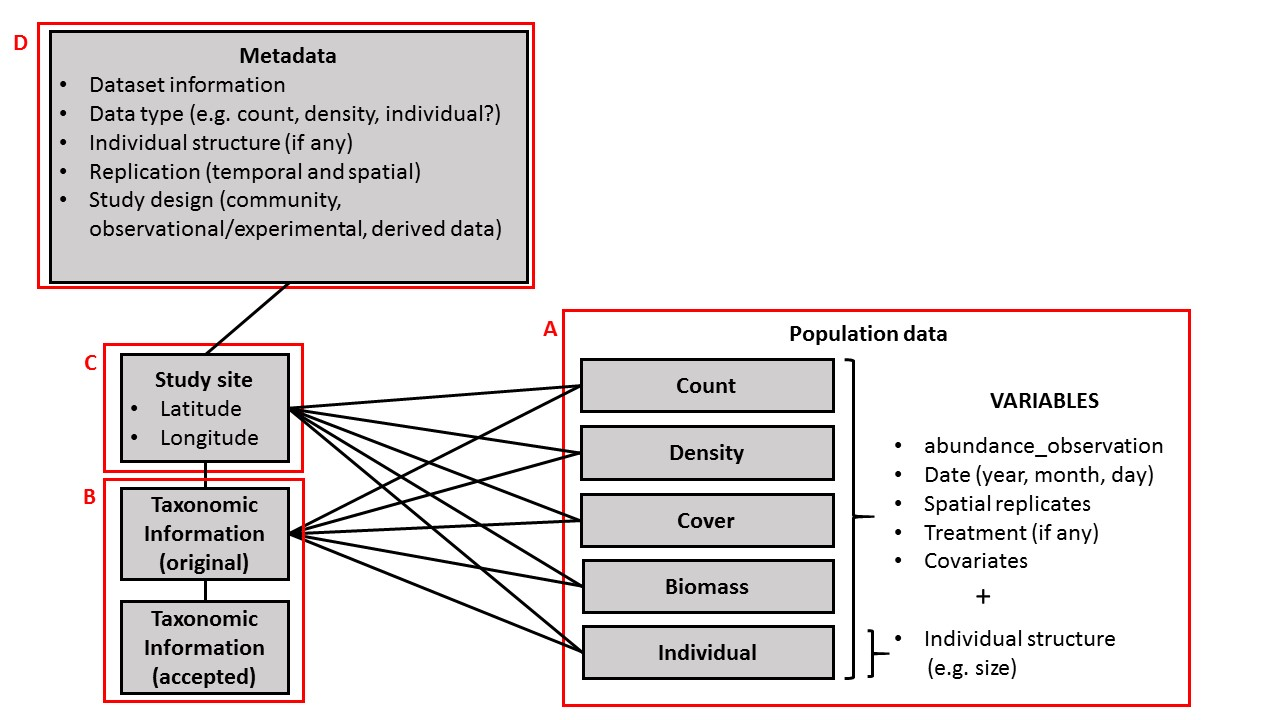
\includegraphics[scale=0.4]{schema}
    \caption{Schematic representation of the entity relationship diagram of the \texttt{popler} database. \texttt{popler} provides metadata on the studies that originated abundance data points (D). This metadata contains information on the unique identifiers of each study, on its design (observational or experimental), temporal and spatial replication. Popler stores the latitude and longitude of the study site (C). Each abundance data point corresponds to a specific taxonomic unit (B). Finally, the time series population data collected in a study can be of five different types: count, density, biomass, cover, and individual data (A).}
    \label{Fig:schema}
  \end{center}
\end{figure}

\newpage
\begin{figure}[h!]
  \begin{center}
    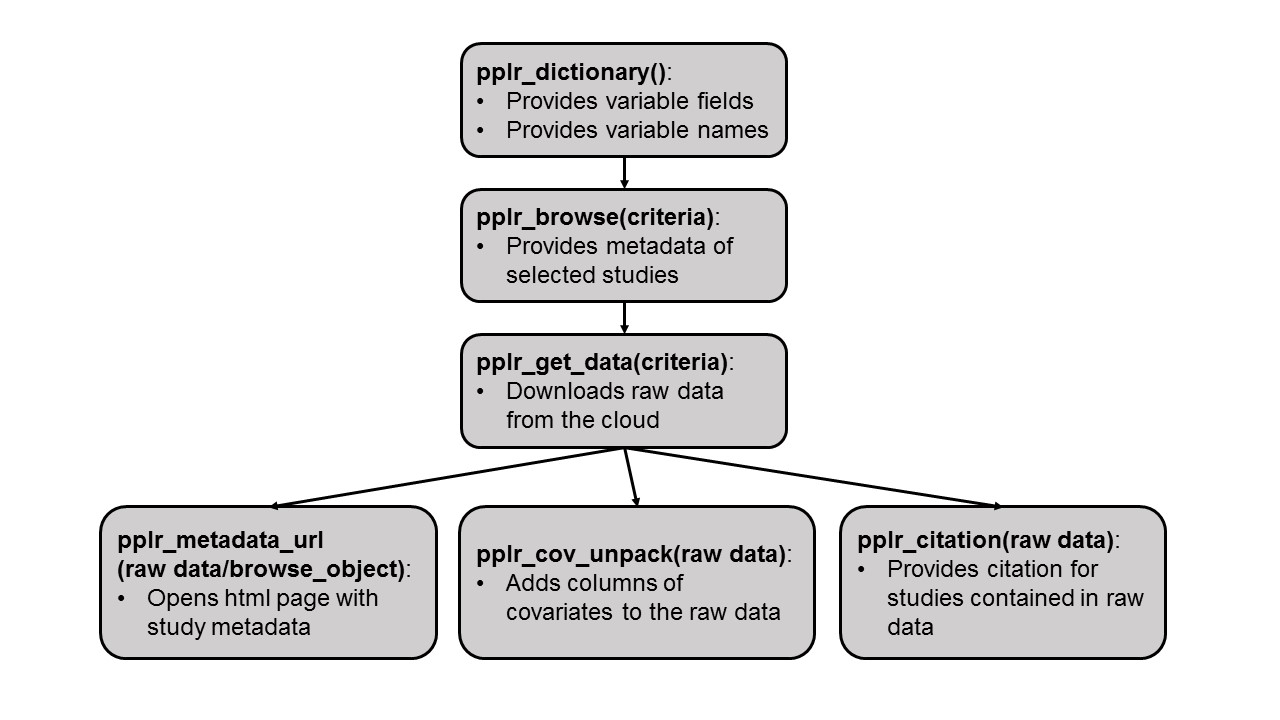
\includegraphics[scale=0.4]{pack_funs}
    \caption{Suggested workflow when using the \texttt{popler} R package to interface with the homonymous online database. The function \texttt{dictionary()} refers to the variables of the metadata that describe the data sets contained in \texttt{popler}. \texttt{dictionary()} describes these variables and returns their possible values. This information advises which criteria to use when subsetting \texttt{popler} The user can provide a criterion (that is, a logical statement) to subset the metadata, using \texttt{browse()}, and download dataset from the cloud using \texttt{get\textunderscore data()}. Moreover, the output of \texttt{get\textunderscore data()} (a data frame) can be the argument of three ancillary functions: \texttt{metadata\textunderscore url()} opens the webpage containing the original dataset and their associated online metadata. \texttt{unpack\textunderscore cov()} can be used to format the covariates contained in a raw data object into separate columns of a data frame. Finally, \texttt{popler\textunderscore citation()} provides a citation for the downloaded data set(s).}
    \label{Fig:pack_funs}
  \end{center}
\end{figure}

\newpage
\begin{figure}[h!]
  \begin{center}
    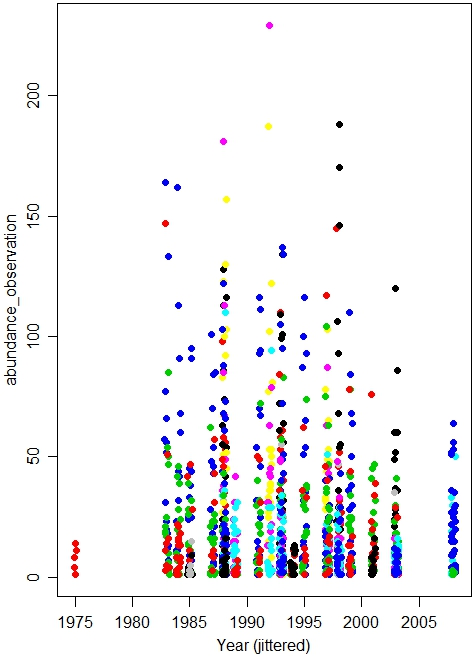
\includegraphics[scale=0.8]{BNZ_plot}
    \caption{Time series of \textit{Viburnum edule} abundance counts at Bonanza Creek LTER. The abundance observation is a count and colors correspond to multiple study sites, the largest scale of spatial replication in \texttt{popler}. There are additional, smaller scales of spatial replication in this study, and hence multiple points per site per year.}
    \label{Fig:BNZ_plot}
  \end{center}
\end{figure}

\newpage
\begin{figure}[h!]
  \begin{center}
    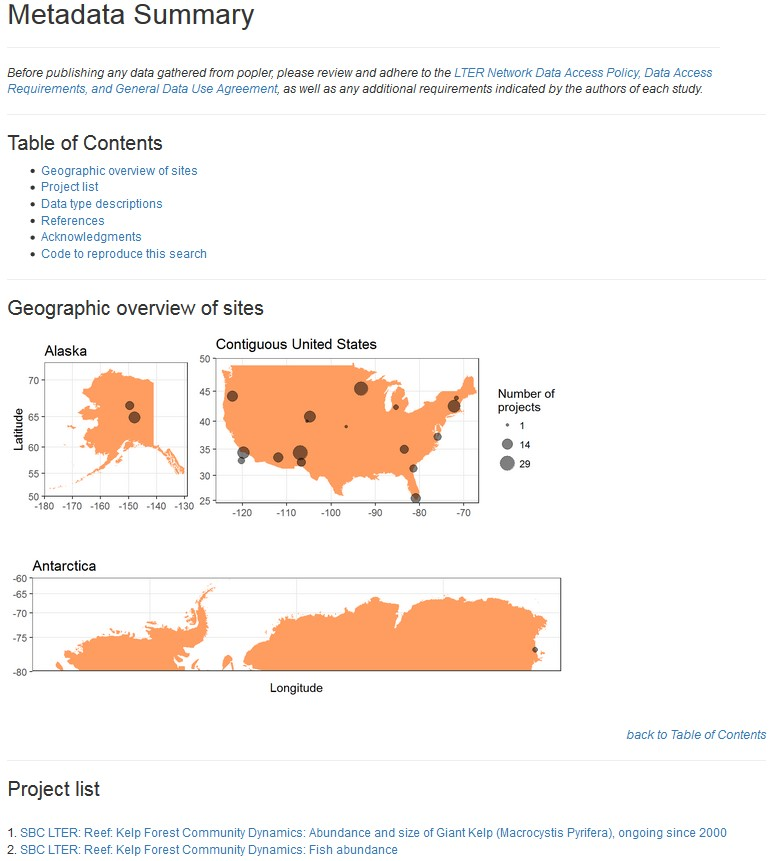
\includegraphics[scale=0.8]{reportT}
    \caption{The html output of function \texttt{browse()} when argument report = TRUE.}
    \label{Fig:reportT}
  \end{center}
\end{figure}

\newpage

\section*{Appendix S1: Pre-processing \texttt{popler} data}
Before uploading datasets into the online \texttt{popler} database, we combined datasets, transformed datasets from wide to long form, converted non-ASCII characters, and modified ambiguous study site names.


The variables of many datasets were contained in two or more separate files, which we combined in a single file. When the original dataset provided data in wide form, we transformed it into long form. In wide form datasets, abundance data associated with different species was stored in separate columns. \texttt{popler} stores these datasets in long form, whereby each row of abundance data is related to a specific taxonomic unit in the table containing taxonomic information (Fig. \ref{Fig:schema}B). We converted all data in ASCII format, because the encoding of the database is the UTF-8. We often re-defined study site names to unambiguously associate them with one of the 26 LTER sites. Many site names are alphanumeric codes (e.g. ``U1'') which can overlap across several LTER sites. Hence, we changed site names following a standard formula (namely, from ``U1'' to ``site\textunderscore sbc\textunderscore U1'', where ``sbc'' refers to the Santa Barbara coastal LTER site).

In a handful of cases, we removed single data rows from the original dataset. These data rows were associated with two types of typos in the original dataset. First, some abundance observations were not associated with a time of observation. We removed this data because \texttt{popler} can only accommodate population information associated with a time of observation. Second, a handful of abundance data points were clear typos (e.g. the letter ``l'' instead of a numeric value). We substituted these data points with a missing value (NULL in the database). We uploaded these pre-processed datasets in the \texttt{popler} database through a Graphic User Interface developed in Python using libraries panda and pyqt5.

\newpage
\setcounter{table}{0}
\renewcommand{\thetable}{S\arabic{table}}

\begin{table}[h!]
  \caption{Taxonomic variables contained in the popler table on original taxonomic information.}
  \label{Tab:S1}
  \begin{center}
    \begin{tabular}{l}
      \hline
      Variable\\
      \hline
      \texttt{sppcode} \\
      \texttt{kingdom}\\
      \texttt{subkingdom}\\
      \texttt{infrakingdom}\\
      \texttt{superdivision}\\
      \texttt{division}\\
      \texttt{subdivision}\\
      \texttt{superphylum}\\
      \texttt{phylum}\\
      \texttt{subphylum}\\
      \texttt{class}\\
      \texttt{subclass}\\
      \texttt{order}\\
      \texttt{family}\\
      \texttt{genus}\\
      \texttt{species}\\
      \texttt{common\textunderscore name}\\
      \hline
    \end{tabular}
  \end{center}
\end{table}



\newpage
\begin{table}[h!]
  \caption{Metadata variables used to describe the datasets stored in \texttt{popler.}}
  \label{Tab:S2}
  \begin{center}
    \begin{tabular}{p{5cm} p{10cm}}
      \hline
      Variable & Description \\
      \hline
\texttt{proj\textunderscore metadat\textunderscore key} & {Unique ID} \\
\texttt{lter\textunderscore project\textunderscore key} & {ID of LTER site} \\
\texttt{lter\textunderscore project\textunderscore key} & {ID of LTER site} \\
\texttt{title} & {Title of study} \\
\texttt{samplingunits} & {Unit of measure (if any) referred to population data.} \\
\texttt{datatype} & {Data type: count, biomass, cover, density, and individual. These correspond to the tables in Fig. \ref{Fig:schema}A.} \\
\texttt{structured\textunderscore type\textunderscore n} & {If individual data, this shows what type of structure is stored. A study can contain up to $n = 4$ types of structure.}\\
\texttt{structured\textunderscore type\textunderscore n\textunderscore units} & {Unit of measure (if any) referred to structure data.}\\
\texttt{studystartyr} & {Start year of the study} \\
\texttt{studyendyr} & {End year of the study} \\
\texttt{duration\textunderscore years} & {Duration of the study in years} \\
\texttt{samplefreq} & {Frequency of population census} \\
\texttt{studytype} & {Whether study is observational or experimental} \\
\texttt{community} & {Whether study includes single taxon (\texttt{community = F}) or multiple taxa (\texttt{community = T})} \\
\texttt{spatial\textunderscore replication\textunderscore level\textunderscore n\textunderscore extent} & {Extent of spatial replication level number $n$. A dataset can have up to to 5 replication levels.} \\
\texttt{spatial\textunderscore replication\textunderscore level\textunderscore n\textunderscore extent\textunderscore units} & {Unit of spatial extent of the $n$ spatial replication level.} \\
\texttt{spatial\textunderscore replication\textunderscore level\textunderscore n\textunderscore label} & {Label of the spatial replication level (e.g. transect, plot, quadrat, ect.). The label of spatial replication level 1 is ``site''.} \\
\texttt{spatial\textunderscore replication\textunderscore level\textunderscore n\textunderscore number\textunderscore of\textunderscore unique\textunderscore reps} & {The number of unique replicates for the $n$th level of spatial replication.} \\
\texttt{treatment\textunderscore type\textunderscore n} & {The type of treatment. \tom{This is vague and does not correspond to level $n$. PROBLEM.}} \\
\texttt{control\textunderscore group} & {If study is experimental, this shows the field(s) that identify the control replicate.} \\
\texttt{derived} & {Is population size data raw, or is it derived (e.g. it is aggregated)?} \\
\texttt{authors} & {Author(s) of the original dataset} \\
\texttt{authors\textunderscore contact} & {Email address(es) of the author(s) associated with the original dataset.} \\
\texttt{metalink} & {url of the original dataset} \\
\texttt{knbid} & {Knowledge Network for Biocomplexity identifier.} \\
      \hline
    \end{tabular}
  \end{center}
\end{table}


\newpage
\begin{table}[h!]
  \caption{LTER identification acronyms and their meaning as used in the \texttt{popler} database.}
  \label{Tab:S3}
  \begin{center}
    \begin{tabular}{l l}
      \hline
      Variable & LTER name\\
      \hline
SBC & Santa Barbara Coastal LTER\\
SEV & Sevilleta LTER \\
SGS & Shortgrass Steppe\\
VCR & Virginia Coastal Reserve LTER\\
AND & Andrew Forest LTER\\
NWT & Niwot Ridge LTER\\
BNZ & Bonanaza Creek LTER\\
CDR & Cedar Creek Ecosystem Science Reserve\\
GCE & Georgia Coastal Ecosystems LTER\\
ARC & Arctic LTER\\
CAP & Central Arizon - Phoneix LTER\\
FCE & Florida Coastal Everglades LTER\\
HFR & Harvard Forest LTER\\
KBS & Kellogg Biological Station LTER\\
CWT & Coweeta LTER\\
HBR & Hubbard Brook LTER\\
MCM & McMurdo Dry Valleys LTER\\
JRN & Jornada Basin LTER\\
CCE & California Current Ecosystem LTER\\
KNZ & Konza Prairie LTER\\
      \hline
    \end{tabular}
  \end{center}
\end{table}

\end{document}
